% Type of the document
\documentclass{beamer}

% elementary packages:
\usepackage{graphicx}
\usepackage[latin1]{inputenc}
\usepackage[T1]{fontenc}
\usepackage[english]{babel}
\usepackage{listings}
\usepackage{xcolor}
\usepackage{eso-pic}
\usepackage{mathrsfs}
\usepackage{url}
\usepackage{amssymb}
\usepackage{amsmath}
\usepackage{multirow}
\usepackage{hyperref}
\usepackage{booktabs}

% additional packages
\usepackage{bbm}

% packages supplied with ise-beamer:
\usepackage{cooltooltips}
\usepackage{colordef}
\usepackage{beamerdefs}
\usepackage{lvblisting}

\begin{document}

%%%%%%%%%%%%%%%%%%%%%%%%%%%%%%%%%%%%%%%%%%%%%%%%%%%%%%%%%%%%%%%%%%%%%%%%%%%%%%%%%%%%%%%%%%%%%%%%%%%%%%%%%%%%%%%%%%%%%%%%
\section{Solution to Quizzes}
%%%%%%%%%%%%%%%%%%%%%%%%%%%%%%%%%%%%%%%%%%%%%%%%%%%%%%%%%%%%%%%%%%%%%%%%%%%%%%%%%%%%%%%%%%%%%%%%%%%%%%%%%%%%%%%%%%%%%%%%
\frame{
\frametitle{Quiz 11: If $X_n$ is $\operatorname{AN}(\mu_n, \sigma_{n}^2)$, then so is $\frac{n-1}{n}X_n$, but NOT $\frac{n^{1/2}-1}{n^{1/2}}X_n$, why? and find a $r.v. X_n s.t. X_n \sim \operatorname{AN}(n, 2n)$}
Proof: \\
According to Lemma 23, if $X_n$ is $\operatorname{AN}(n, 2n)$, then also $a_nX_n+b_n$ is 
$\operatorname{AN}(n, 2n) \iff a_n \rightarrow 1, \frac{\mu_n(a_n-1)+b_n}{\sigma_n} \rightarrow 0$.
\begin{itemize}
\item For $\frac{n-1}{n}X_n$:\\
$a_n=\frac{n-1}{n}, b_n=0,$ we have obviously \\
$a_n=\frac{n-1}{n} \rightarrow 1, \frac{\mu_n(a_n-1)+b_n}{\sigma_n}=\frac{n(\frac{n-1}{n}-1)+0}{\sqrt{2n}}=\frac{-1}{\sqrt{2n}}\rightarrow 0$\\
By Lemma 23, $\frac{n-1}{n}X_n$ is also $\operatorname{AN}(n, 2n)$.
\end{itemize} }
}

\frame{
\frametitle{Quiz 11: If $X_n$ is $\operatorname{AN}(\mu_n, \sigma_{n}^2)$, then so is $\frac{n-1}{n}X_n$, but NOT $\frac{n^{1/2}-1}{n^{1/2}}X_n$, why? and find a $r.v. X_n s.t. X_n \sim \operatorname{AN}(n, 2n)$}
Proof:\\
\begin{itemize}
\item For $\frac{n^{1/2}-1}{n^{1/2}}X_n$:\\
$a_n=\frac{n^{1/2}-1}{n^{1/2}}, b_n=0,$ we have obviously\\
$a_n=\frac{n^{1/2}-1}{n^{1/2}} \rightarrow 1, \frac{\mu_n(a_n-1)+b_n}{\sigma_n}=\frac{n(\frac{n^{1/2}-1}{n^{1/2}}-1)+0}{\sqrt{2n}}=-\sqrt{2}/2 \nrightarrow 0$\\
By Lemma 23, $\frac{n^{1/2}-1}{n^{1/2}}$ is not $\operatorname{AN}(n, 2n)$.
\end{itemize} 
}

\frame{
\frametitle{Quiz 11: If $X_n$ is $\operatorname{AN}(\mu_n, \sigma_{n}^2)$, then so is $\frac{n-1}{n}X_n$, but NOT $\frac{n^{1/2}-1}{n^{1/2}}X_n$, why? and find a $r.v. X_n s.t. X_n \sim \operatorname{AN}(n, 2n)$}
An example $r.v. X_n$ satisfies $X_n \sim \operatorname{AN}(n, 2n)$
\begin{center}
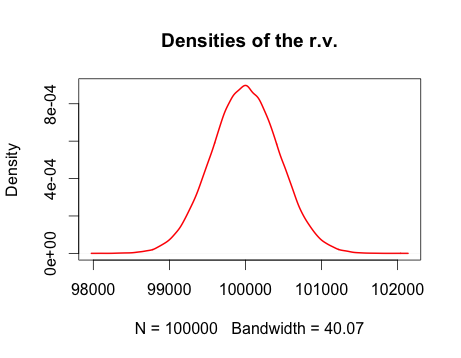
\includegraphics[scale=0.35]{MSM_AN.png}
\end{center}
	\begin{center}	\href{https://github.com/xuxiu/MSMquiz/tree/master/Quiz11_p5-15}{\quantnet Quiz11-MSM.R}
    \end{center}
}

\end{document}